\section{Motorsteuerung}
	Dem Roboter stehen 2 starke gro\ss{}e und ein schw"acherer mittelgro\ss{}er Motor zur Verf"ugung.\\ \\
	\begin{figure}[h]
		\begin{floatrow}
			\ffigbox{%
				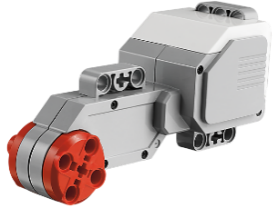
\includegraphics[width=4cm]{images/bigMotor.png}%\rule{3cm}{3cm}%
			}{%
				\caption{gro\ss{}er Motor}%
			}
			\ffigbox{%
				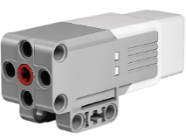
\includegraphics[width=4cm]{images/mediumMotor.png}%\rule{3cm}{3cm}%
				
			}{%
				\caption{mittlerer Motor}%
			}
		\end{floatrow}
	\end{figure}

	
	
	\begin{table}[h]
		\begin{tabular}{|p{0.2\textwidth}| p{0.7\textwidth}|}
			\hline
			Motorausgang & lejos.hardware.port.MotorPort\\ \hline
			gro\ss{}er Motor& lejos.hardware.motor.EV3LargeRegulatedMotor
			 \\ \hline mittlerer Motor & lejos.hardware.motor.EV3LargeMediumRegulatedMotor\\ \hline 
		\end{tabular}
		\caption{ben"otigte Imports}
	\end{table}
 
	\begin{table}[H]
		\begin{tabular}{|p{0.2\textwidth}| p{0.7\textwidth}|}
			\hline
			forward()& Motor dreht sich vorw"arts \\ \hline 
			backward() &  Motor dreht sich r"uckw"arts\\ \hline 
			stop() & Motor stoppt\\ \hline
			rotate(int a) & Motor dreht sich um a Grad\\ \hline
			setSpeed(int x) & setzt die Geschwindigkeit des Motors \\
			& Das Maximum ist hierbei 800\\ \hline
		\end{tabular}
		\caption{wichtige Methoden}
	\end{table}

	Um die Motoren verwenden zu k"onnen, muss zuerst der Motorport und der entsprechende Motor oben in der Datei importiert werden.\\ 
	\textbf{Bsp.: import lejos.hardware.motor.EV3LargeRegulatedMotor;}\\ \\
	Als n"achstes muss 
	Im folgenden Beispiel steht \glqq name\grqq{} f"ur einen frei w"ahlbaren Namen und \glqq X\grqq{} f"ur den Port, also A, B, C oder D.\\
	\textbf{EV3LargeRegulatedMotor name = new EV3LargeRegulatedMotor(MotorPort.X);} \\ 
	\textbf{Bsp.: EV3LargeRegulatedMotor motor = new EV3LargeRegulatedMotor(MotorPort.A);}\\ \\
	Damit sich der Motor bewegt, m"ussen dem Motor nach folgendem Muster eine der gegebenen Methoden gegeben werden.\\
	\textbf{name.Methode;}\\
	\textbf{Bsp.: motor.forward();}

	